\section{Decentralized Language Models (\toolName{})}
\label{sec:method}

\begin{figure}
    \centering
    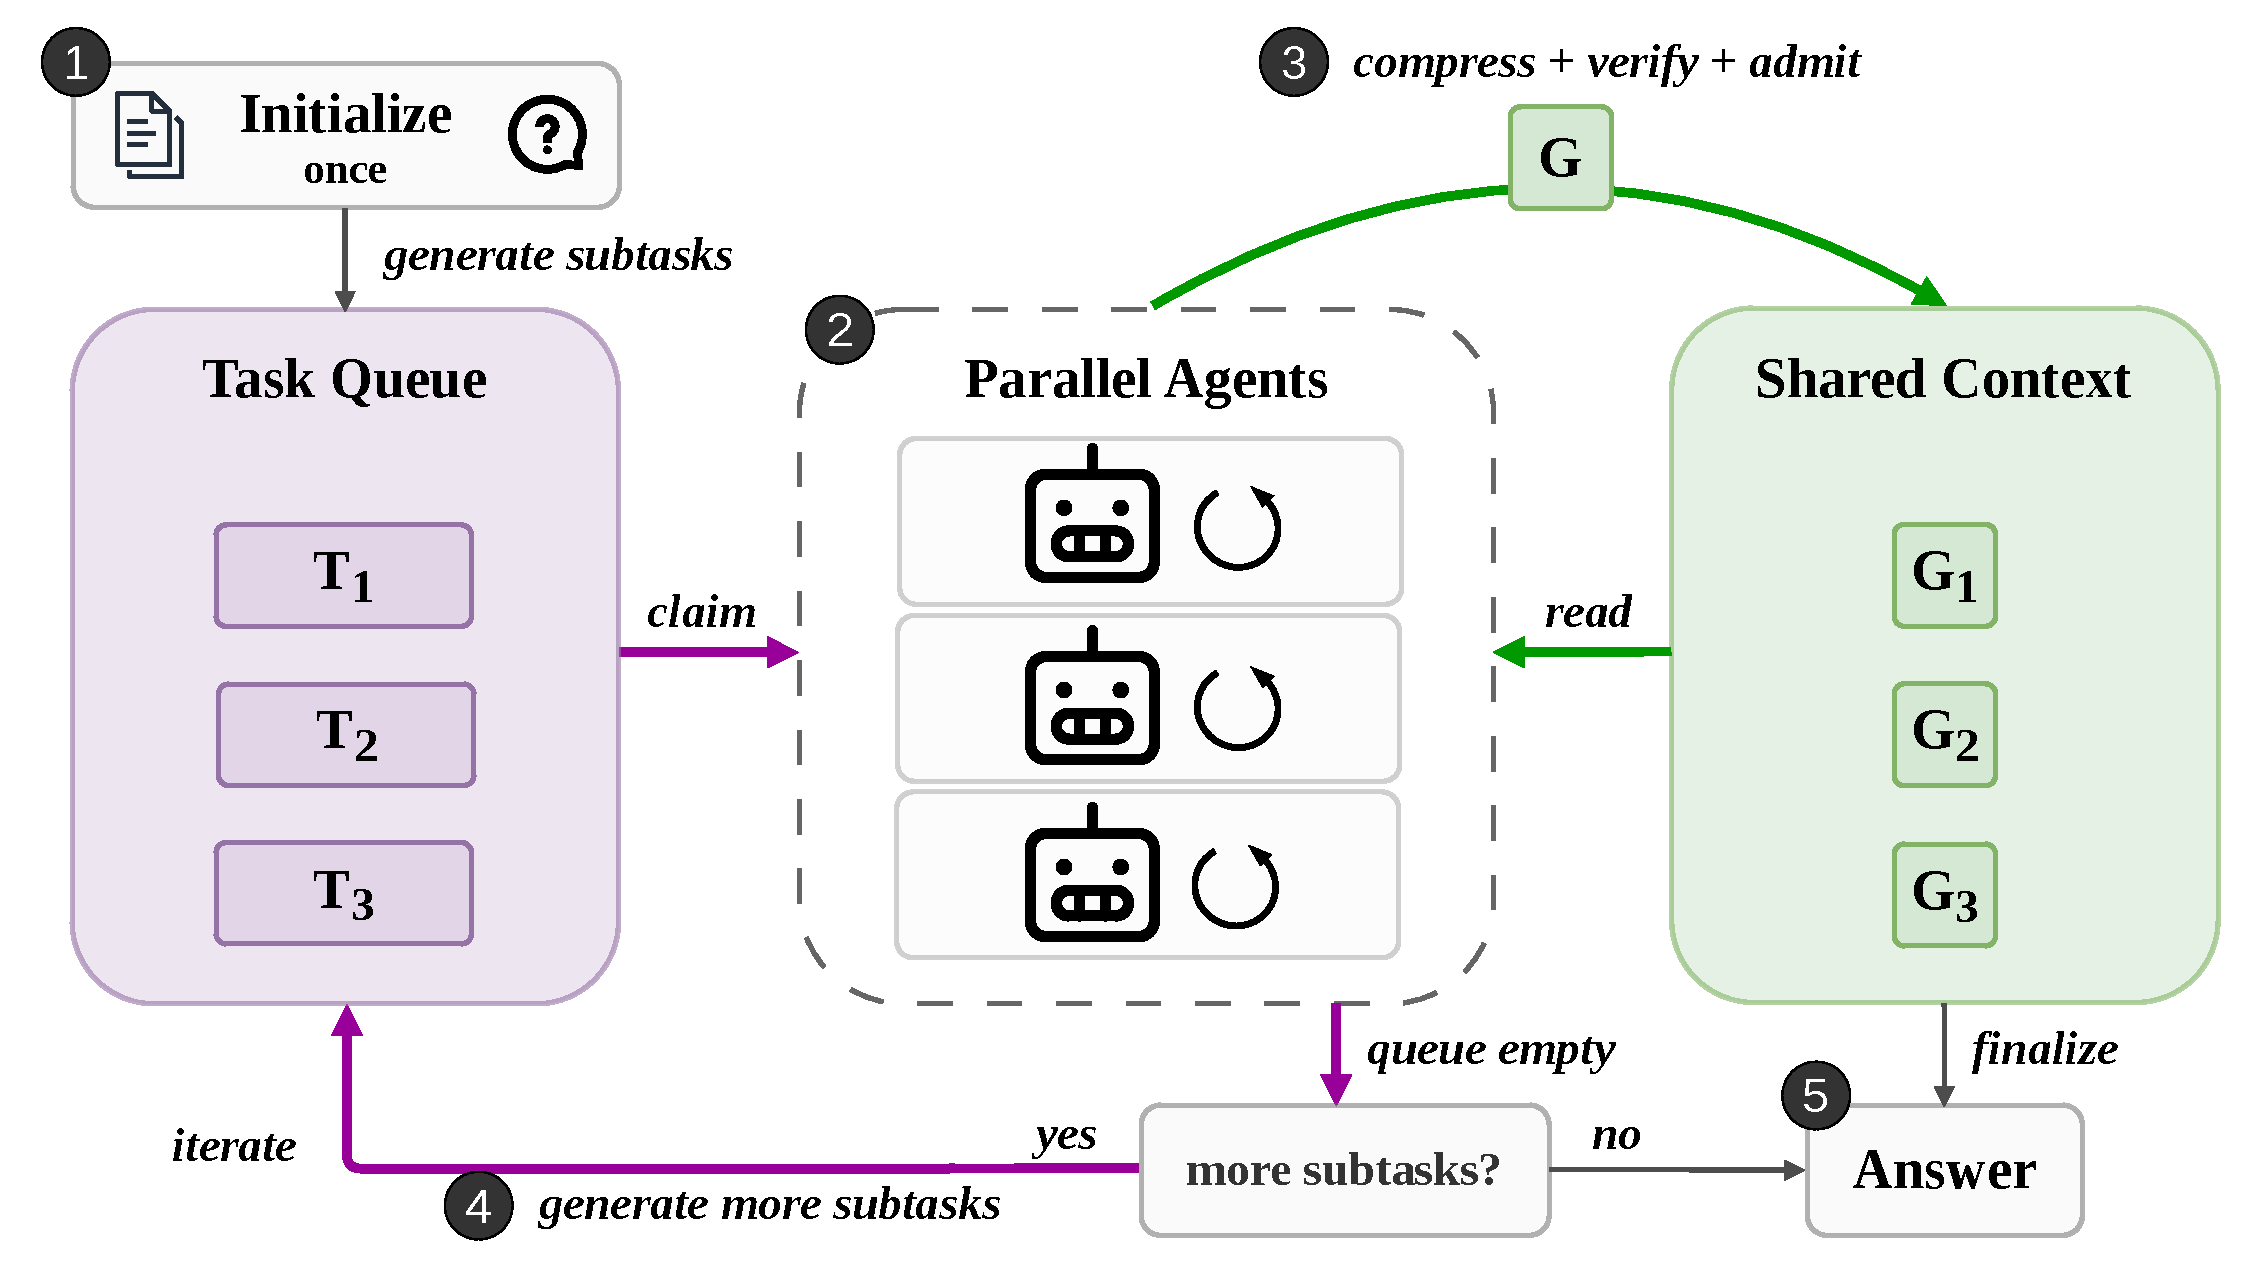
\includegraphics[width=1\linewidth]{pipe.pdf}
    \caption{\textbf{Overview of \toolName{}.} A one-time initialization step decomposes the input into initial subtasks and places them in a shared task queue. Parallel agents asynchronously claim tasks (${T_i}$), read the verified shared context, and perform local reasoning. Completed updates are compressed, verified, and admitted as compact gists ({${G_i}$}), making reusable progress visible to all agents. When the task queue becomes empty, the most recently completed agent checks the existing subtask states and shared context to decide whether additional subtasks are needed. If so, it generates and enqueues new tasks for another round of parallel execution; otherwise, it produces the final answer.
}
    \label{fig:pipeline}
\end{figure}

\begin{algorithm}
\caption{\textbf{\toolName{} pipeline.} \toolName{} maintains a shared context $\sctx$ and a task queue $\tque$. Agents execute queued subtasks in parallel, compress and verify their results $\{r_i\}$ into compact gists, admit verified gists to the shared context, optionally generate additional subtasks from accumulated state, and finally produce the answer from the verified shared context.}
\label{alg:dlm}
\begin{algorithmic}[1]
\Require Task $D$; optional source context $U$
\Ensure  Final answer $Y$

\State $\sctx \gets \emptyset$ \Comment{shared context}
\State $\tque \gets \Call{GenerateSubtasks}{D, U}$ \stage{1}

\Repeat
    \State $\{r_i\} \gets \Call{RunAgents}{\tque, \sctx}$ \stage[\Comment{execute subtasks in parallel}]{2}
    \State $\{G_i\} \gets \Call{CompressAndVerify}{\{r_i\}}$ \stage{3}
    \State $\sctx \gets \sctx \cup \{G_i\}$ \Comment{admit verified gists}

    \If{$\tque$ is empty}
        \State $\tque \gets \Call{GenerateMoreSubtasks}{D, \sctx}$ \stage{4}
    \EndIf
\Until{$\tque$ is empty}

\State $Y \gets \Call{Finalize}{D, \sctx}$ \stage{5}
\State \Return $Y$
\end{algorithmic}
\end{algorithm}

\toolName{} implements these design principles through two global structures: a shared context $\sctx$ and a task queue $\tque$. Given an input task $D$ and optional source context $U$, $\sctx$ stores compact, verified gists of accumulated progress, while $\tque$ stores pending subtasks for parallel execution.

As shown in Figure~\ref{fig:pipeline} and Algorithm~\ref{alg:dlm}, \toolName{} proceeds in five stages\mbox{: \stage{1}}~initialize the task queue from the input\mbox{, \stage{2}}~execute ready subtasks in parallel\mbox{, \stage{3}}~compress, verify, and admit updates into the shared context\mbox{, \stage{4}}~generate additional subtasks when the current shared context is insufficient, \mbox{and \stage{5}} produce the final answer once no further subtasks are needed. We next describe the two core mechanisms underlying this pipeline: Section~\ref{sec:shared_context} introduces the shared context and task queue, and Section~\ref{sec:compression_verification} describes how intermediate updates are compressed, verified, and admitted.

% This separation between a fixed loop and pluggable components is what makes \toolName{} modular: every \plug{highlighted} call site in Algorithm~\ref{alg:pipeline}---the summarizers $\phi_1, \phi_2$, the verifiers \textsc{Verify-U/T}, the planner \textsc{Plan}/\textsc{Replan}, the per-task worker \textsc{RunAgent}, and the finalizer \textsc{Finalize}---is a pluggable component that can be adapted to new domains without changing the pipeline.


\subsection{Shared Context and Task Queue}
\label{sec:shared_context}
\toolName{} maintains two global structures: a shared context $\sctx$ and a task queue $\tque$. The shared context stores compact, reusable problem state, including source evidence, completed subtask results, failed hypotheses, and intermediate constraints. The task queue stores pending subtasks that available agents can claim in parallel. Together, $\sctx$ and $\tque$ define the coordination interface: agents choose work from $\tque$ and communicate progress through admitted entries in $\sctx$.

The key design choice is that $\sctx$ contains gist entries $G_i$ rather than raw traces. Each gist summarizes information useful for future agents and points to more detailed evidence that can be retrieved through selective unfolding. Thus, every worker can read a lightweight global view of the current problem state without losing access to the underlying details.

The task queue determines how agents act on the shared state. Agents claim ready subtasks from $\tque$ asynchronously; after a gist is admitted into $\sctx$, later agents can build on the finding, avoid a falsified hypothesis, or reuse a partial solution without waiting for a central controller to redistribute it. When the queue is exhausted, the most recently completed agent uses the current subtask states and shared context to determine whether further subtasks are needed. If so, it generates and enqueues new subtasks conditioned on $\tque$ and $\sctx$; otherwise, it finalizes the answer from the accumulated shared state. Appendix~\ref{sec:orchestration} provides further details on dependency-aware
queueing, parallel execution, and systems optimizations


\subsection{Compression and Verified Admission}
\label{sec:compression_verification}
\toolName{} treats each shared-context update as an admission problem. Rather than writing raw agent outputs or unverified summaries directly into $\sctx$, it first compresses each completed result into a reusable gist and verifies that gist against its supporting evidence. Only updates that pass this gate become visible to other agents.

Specifically, given a completed result $r_i$, \toolName{} chooses the compression path based on the type of content being admitted. If $r_i$ is a reasoning trajectory, it may contain a successful finding, a falsified hypothesis, execution feedback, or a constraint for future agents. Since later agents usually need the distilled conclusion rather than the full trace, \toolName{} directly compresses $r_i$ into a gist $G_i$. If $r_i$ is a long source unit, however, direct gist-to-raw unfolding can be unreliable: the gist may not preserve enough detail to identify the exact raw span to unfold, while unfolding many candidate chunks to compensate is expensive. \toolName{} therefore uses a hierarchical path, $r_i \rightarrow S_i \rightarrow G_i$: it first constructs a reference-grounded summary $S_i$, then compresses $S_i$ into the compact gist $G_i$ admitted to $\sctx$. Both $S_i$ and the raw content remain in backing stores and can be recovered through selective unfolding. Appendix~\ref{sec:summarization} and Appendix~\ref{sec:unfold} give the full hierarchy and unfolding procedure, and Section~\ref{sec:longbench_ablation} validates this design through the ``No Hierarchical Summary'' ablation.


In operating-system terms, the gist layer functions as the small, always-resident working set visible to every agent, while $S_i$ and the raw store serve as backing storage. Selective unfolding acts like demand paging, loading finer-grained evidence into an agent's context only when the current subtask requires it.

Verification follows the same two paths. For a reasoning trajectory, \toolName{} checks whether the gist $G_i$ faithfully captures the relevant finding, failure, feedback, or constraint in $r_i$ using an LLM verifier. For a long source unit, verification is performed at both levels: the summary $S_i$ must be supported by the raw source, and the gist $G_i$ must preserve the supported claims and important qualifiers from $S_i$. Gists that pass are appended to $\sctx$ and become visible to later agents; gists that fail are rejected, regenerated with feedback. Appendix~\ref{sec:verification} gives the full admission-time verification procedure.

% This summarization procedure and admission-time gate turn the shared context from a raw message buffer into curated system state.